\cleardoublepage
\section{Semi-Parametric GPR Models}

In this section the results of the GPR models for two muscles is shown. Figure \ref{fig:GPRMuscleLowerPectoralis} represents Lower Pectoralis and Figure \ref{fig:GPRMuscleTriceps} represents the Triceps. The rest of the Figures for the rest of the muscles can be found in the github repository under the Data/ModelFigures file. 

The figures illustrate a comparison between the parametric and semiparametric models derived from Gaussian Process Regression (GPR) for various muscles across the five arm configurations. The parametric model serves as the foundational representation, built solely on predefined mathematical structures that capture the general tendencies of the data. Consequently, its predictive nature tends to exhibit higher variance since it might not fully grasp all the nuanced details or irregularities inherent in the biological data. In contrast, the semiparametric model, while preserving the core structure of the parametric model, introduces flexible, non-parametric components. By harnessing insights from the parametric data, the semiparametric model becomes more tailored and capable of adapting to specific data peculiarities.

Each plot presents:
\begin{itemize}
    \item The actual test outputs (in blue).
    \item The predicted test outputs (in red dashed lines).
    \item A shaded region representing a confidence interval (±2 standard deviations) around the predicted values.
\end{itemize}

The efficiency of the models were tested by computing the feasibility of 960 generated points (Figure \ref{fig:960 points}). A point was considered feasible if the static controller developed on Section \ref{NeuralController} was able to calculate the corresponding neural activations that will hold the arm in that position for 1 second. The static controller was able to find the neural excitations for 74.06\% of the points. The GIF \ref{gif:Feasiblepoints} shows in green the feasible points and in red the non-feasible ones.

\begin{figure}[h!]
    \centering
   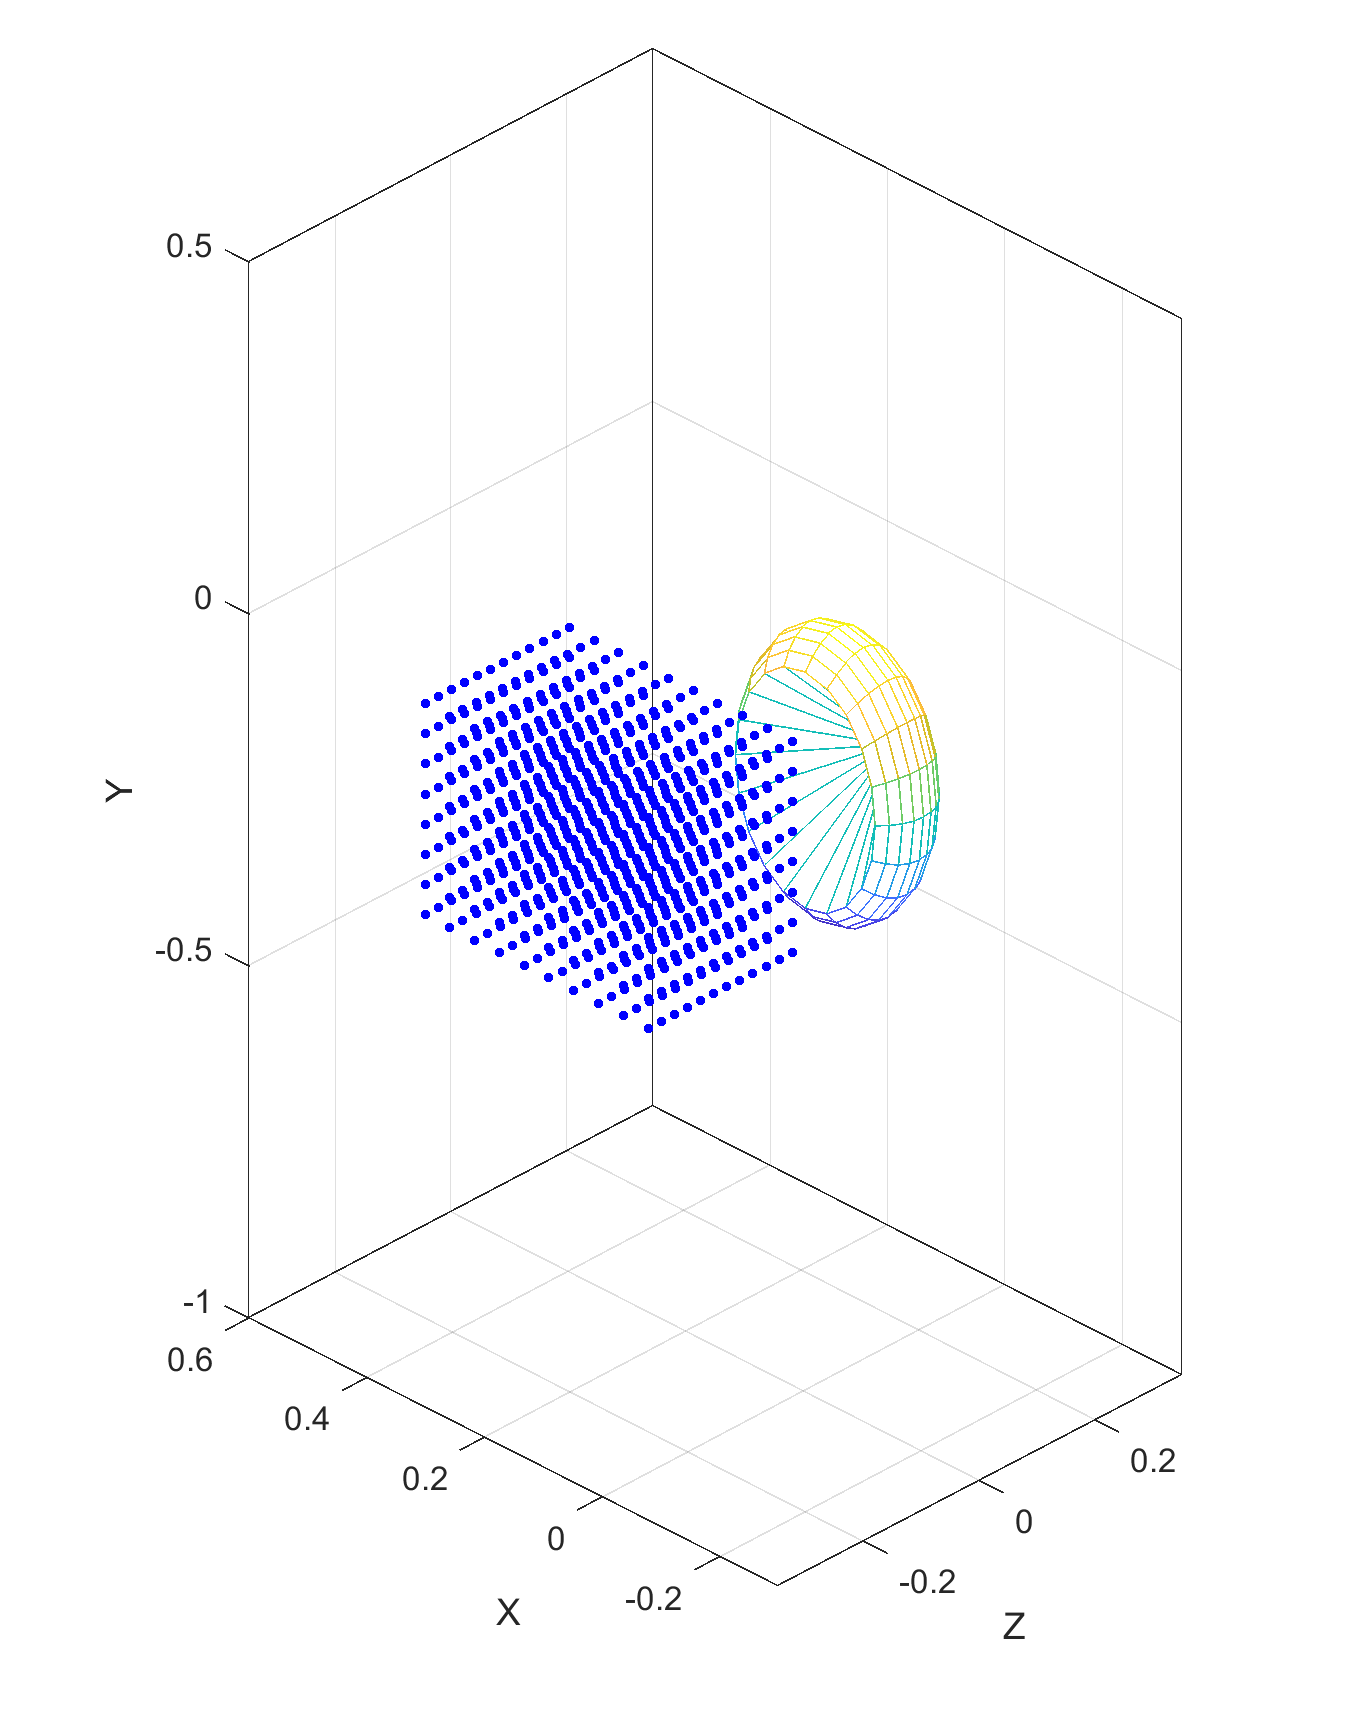
\includegraphics[width=0.4\linewidth]{Pictures/Results/960points.png}
    \caption{960 generated points}
    \label{fig:960 points}
\end{figure}

\begin{figure}[htbp]
    \centering
    % Group 1: elbow pronation
    \begin{subfigure}[b]{0.45\linewidth}
        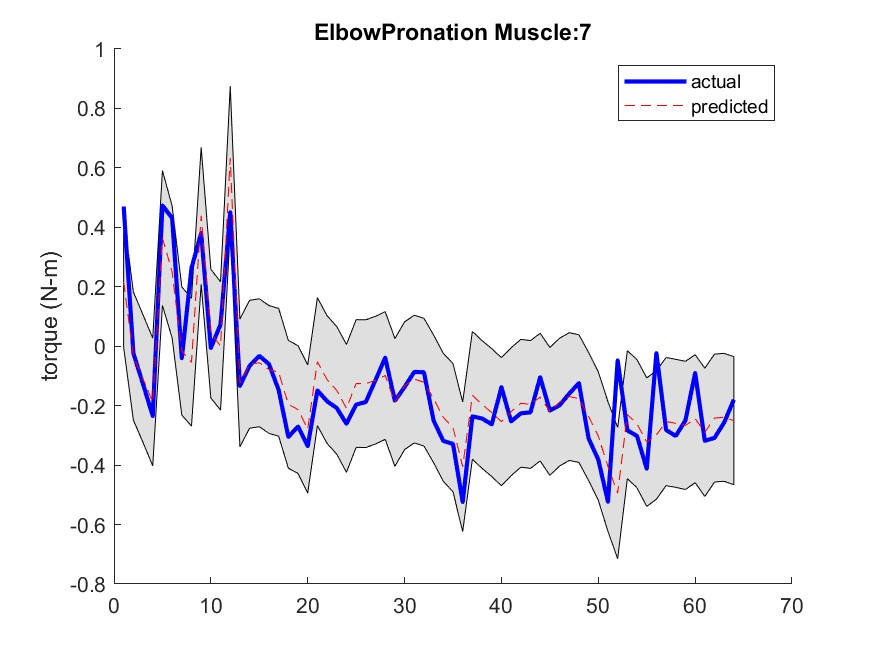
\includegraphics[height=0.15\textheight]{Pictures/Results/GPR/ElbowPronation_7Parametric.jpg}
        \caption{Elbow Pronation Parametric}
    \end{subfigure}
    \hfill
    \begin{subfigure}[b]{0.45\linewidth}
        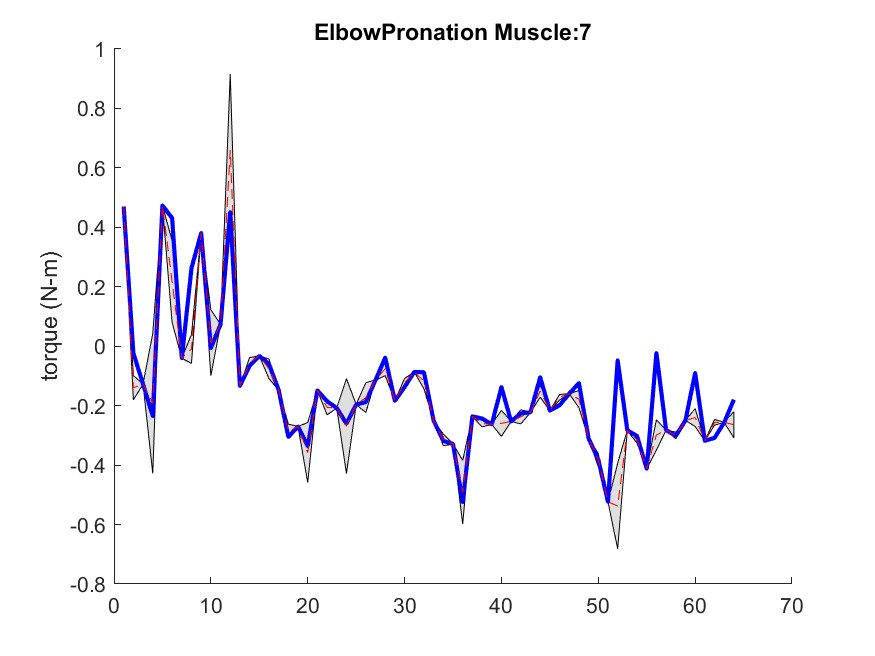
\includegraphics[height=0.15\textheight]{Pictures/Results/GPR/ElbowPronation_7Semiparametric.jpg}
        \caption{Elbow Pronation Semi-parametric}
    \end{subfigure}
    
    % Group 2: elbow flexion
    \begin{subfigure}[b]{0.45\linewidth}
        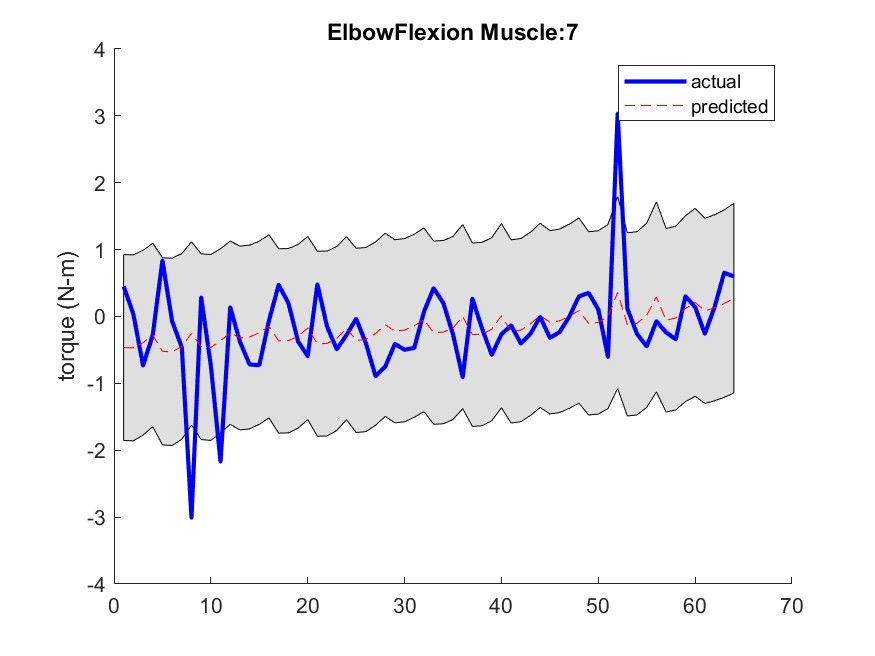
\includegraphics[height=0.15\textheight]{Pictures/Results/GPR/ElbowFlexion_7Parametric.jpg}
        \caption{Elbow Flexion Parametric}
    \end{subfigure}
    \hfill
    \begin{subfigure}[b]{0.45\linewidth}
        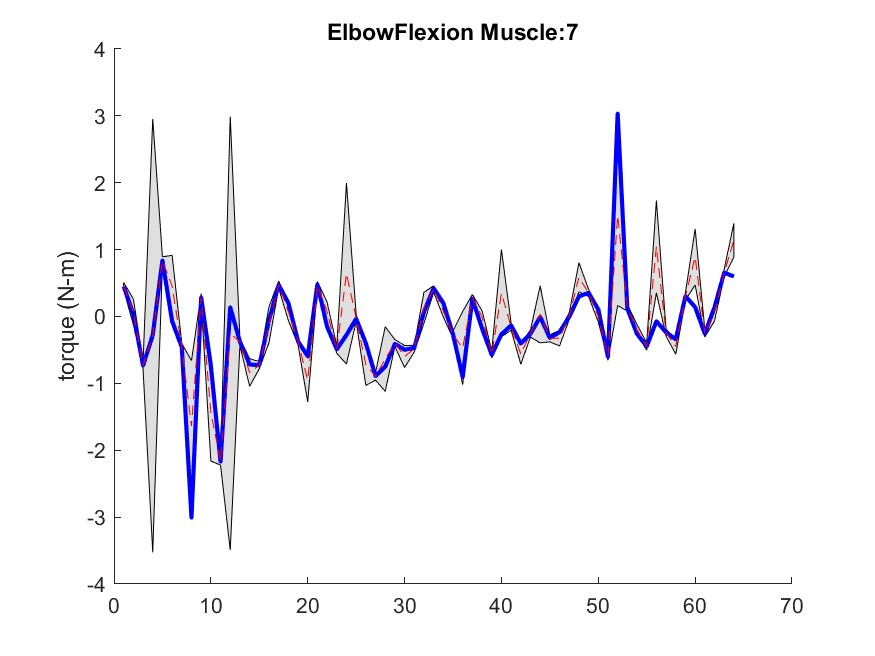
\includegraphics[height=0.15\textheight]{Pictures/Results/GPR/ElbowFlexion_7Semiparametric.jpg}
        \caption{Elbow Flexion Semi-parametric}
    \end{subfigure}
    
    % Group 3: shoulder rotation
    \begin{subfigure}[b]{0.45\linewidth}
        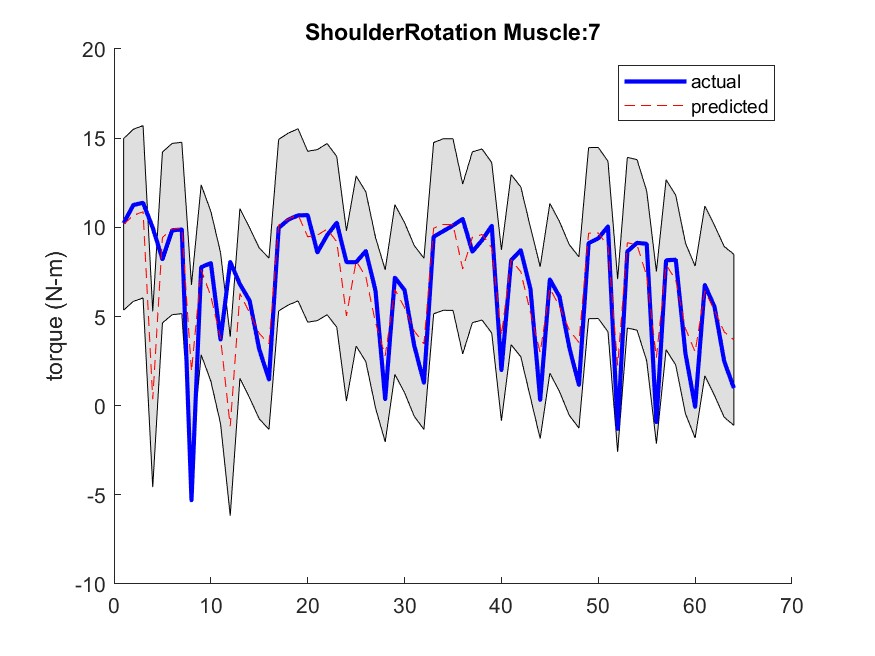
\includegraphics[height=0.15\textheight]{Pictures/Results/GPR/ShoulderRotation_7Parametric.jpg}
        \caption{Shoulder Rotation Parametric}
    \end{subfigure}
    \hfill
    \begin{subfigure}[b]{0.45\linewidth}
        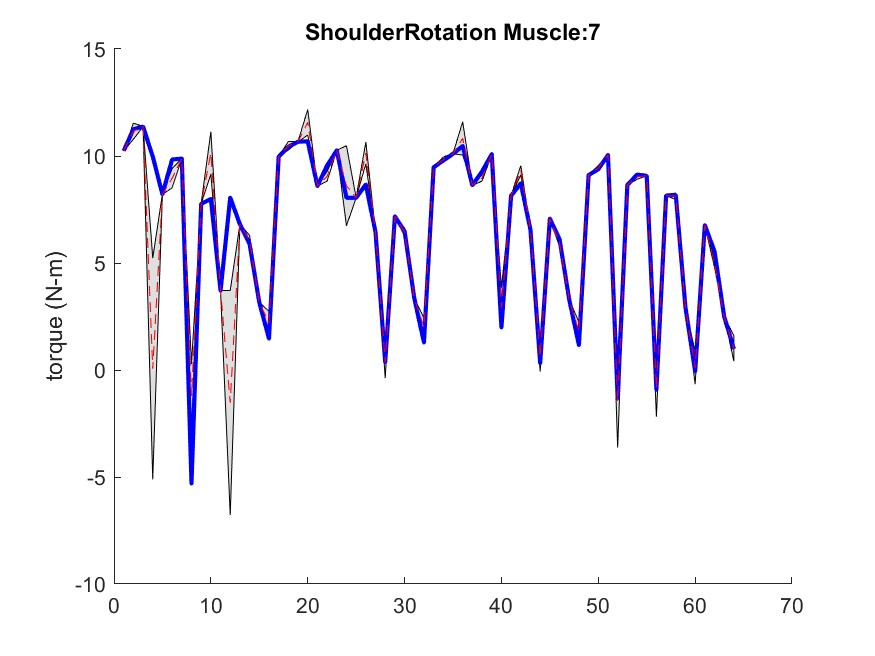
\includegraphics[height=0.15\textheight]{Pictures/Results/GPR/ShoulderRotation_7Semiparametric.jpg}
        \caption{Shoulder Rotation Semi-parametric}
    \end{subfigure}
    
    % Group 4: shoulder elevation
    \begin{subfigure}[b]{0.45\linewidth}
        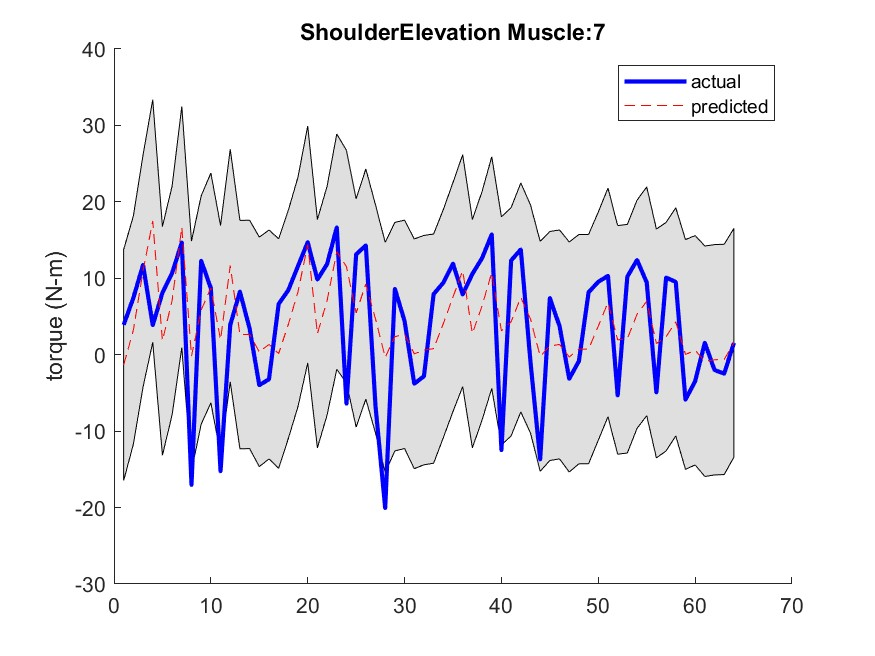
\includegraphics[height=0.15\textheight]{Pictures/Results/GPR/ShoulderElevation_7Parametric.jpg}
        \caption{Shoulder Elevation Parametric}
    \end{subfigure}
    \hfill
    \begin{subfigure}[b]{0.45\linewidth}
        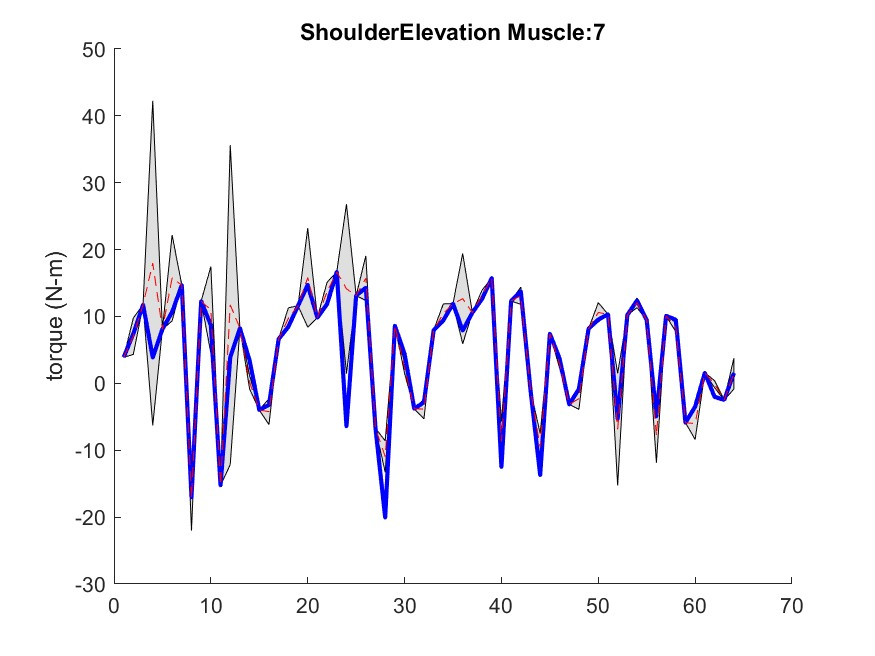
\includegraphics[height=0.15\textheight]{Pictures/Results/GPR/ShoulderElevation_7Semiparametric.jpg}
        \caption{Shoulder Elevation Semi-parametric}
    \end{subfigure}
    
    % Group 5: shoulder elevation plane
    \begin{subfigure}[b]{0.45\linewidth}
        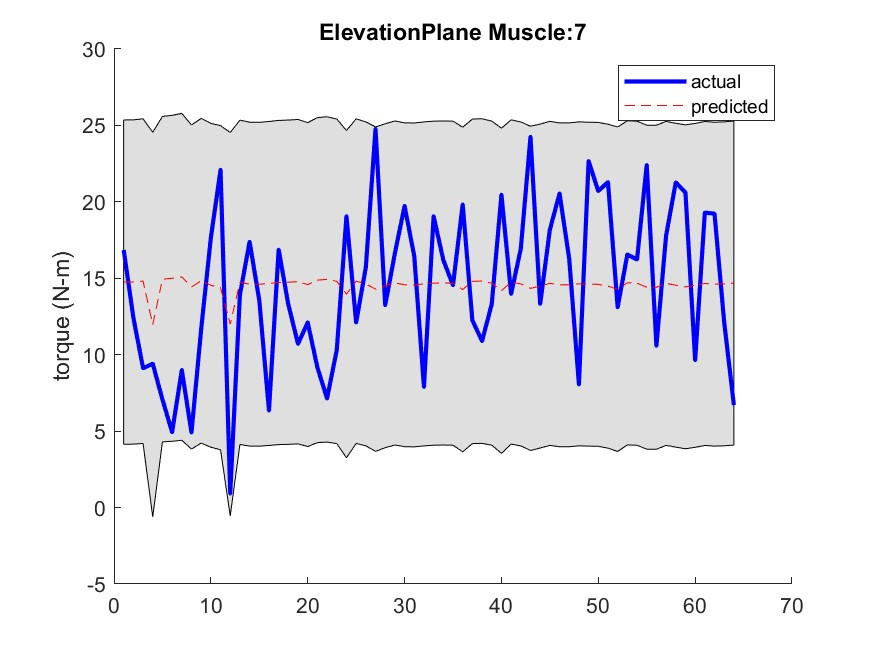
\includegraphics[height=0.15\textheight]{Pictures/Results/GPR/ElevationPlane_7Parametric.jpg}
        \caption{Elevation Plane Parametric}
    \end{subfigure}
    \hfill
    \begin{subfigure}[b]{0.45\linewidth}
        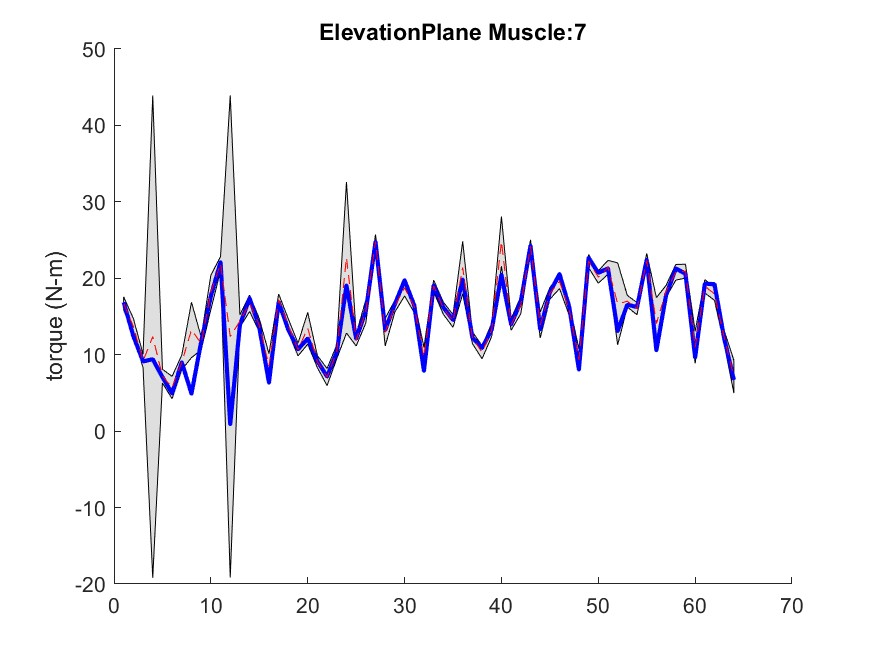
\includegraphics[height=0.15\textheight]{Pictures/Results/GPR/ElevationPlane_7Semiparametric.jpg}
        \caption{Elevation Plane Semi-parametric}
    \end{subfigure}
    
    \caption{Gaussian Process Regression Parametric and Semi-Parametric for Muscle Lower Pectoralis}
    \label{fig:GPRMuscleLowerPectoralis}
\end{figure}

\begin{figure}[htbp]
    \centering
    % Group 1: elbow pronation
    \begin{subfigure}[b]{0.45\linewidth}
        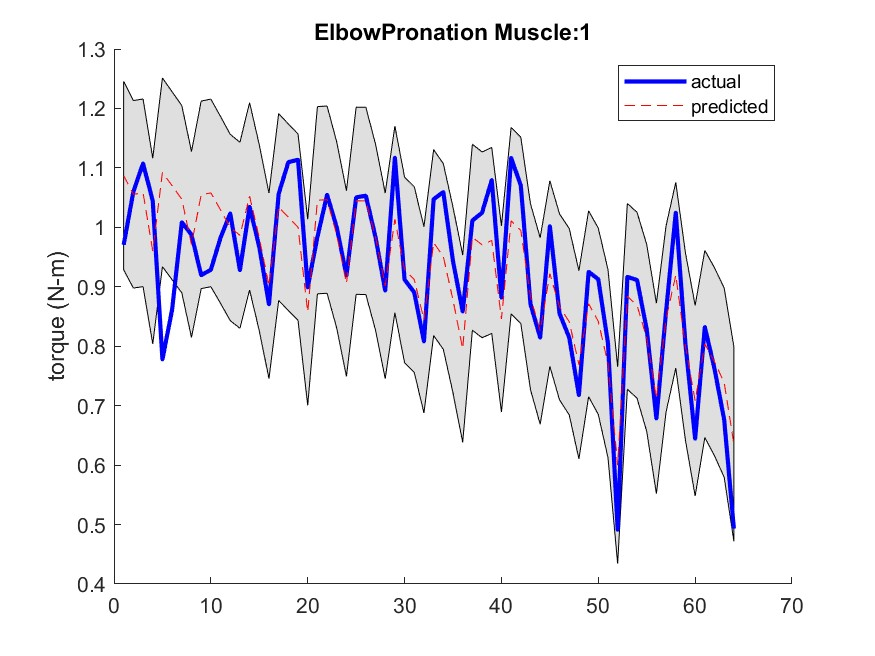
\includegraphics[height=0.15\textheight]{Pictures/Results/GPR/ElbowPronation_1Parametric.jpg}
        \caption{Elbow Pronation Parametric}
    \end{subfigure}
    \hfill
    \begin{subfigure}[b]{0.45\linewidth}
        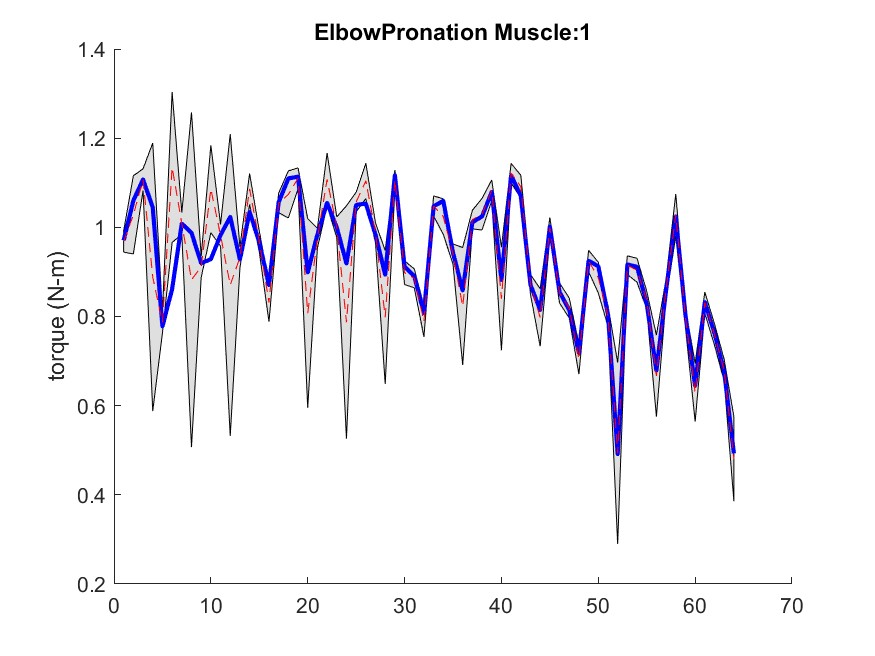
\includegraphics[height=0.15\textheight]{Pictures/Results/GPR/ElbowPronation_1Semiparametric.jpg}
        \caption{Elbow Pronation Semi-parametric}
    \end{subfigure}
    
    % Group 2: elbow flexion
    \begin{subfigure}[b]{0.45\linewidth}
        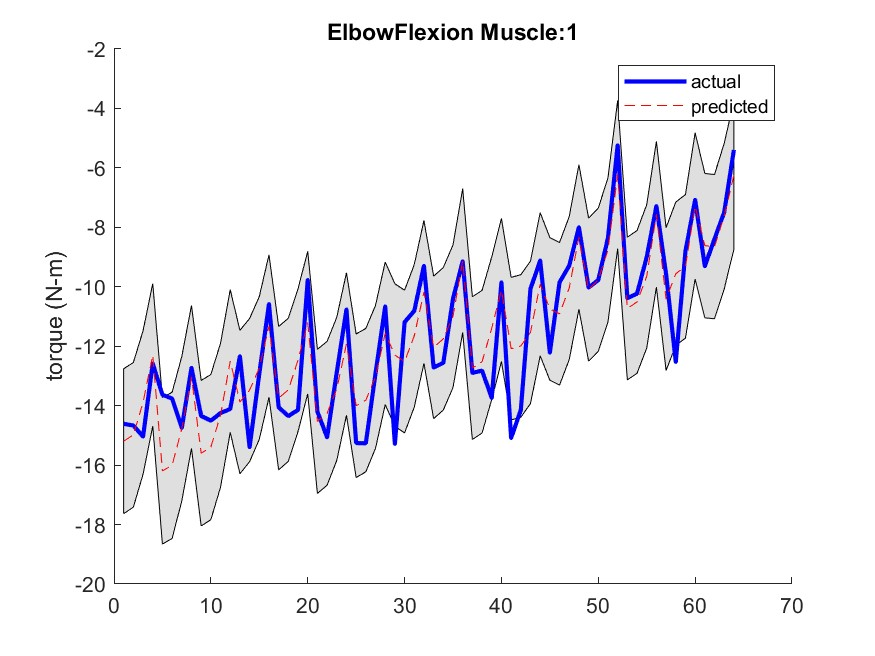
\includegraphics[height=0.15\textheight]{Pictures/Results/GPR/ElbowFlexion_1Parametric.jpg}
        \caption{Elbow Flexion Parametric}
    \end{subfigure}
    \hfill
    \begin{subfigure}[b]{0.45\linewidth}
        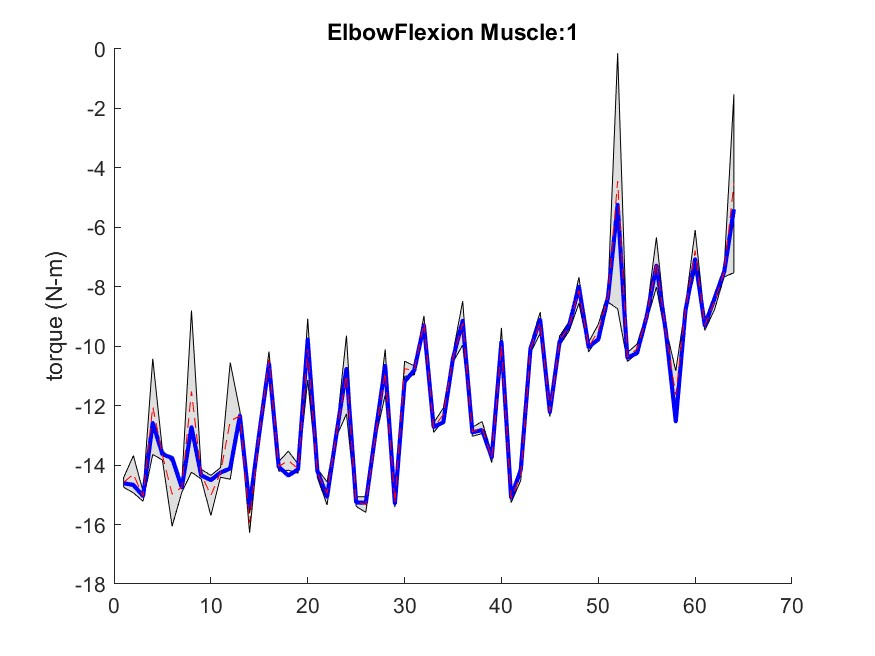
\includegraphics[height=0.15\textheight]{Pictures/Results/GPR/ElbowFlexion_1Semiparametric.jpg}
        \caption{Elbow Flexion Semi-parametric}
    \end{subfigure}
    
    % Group 3: shoulder rotation
    \begin{subfigure}[b]{0.45\linewidth}
        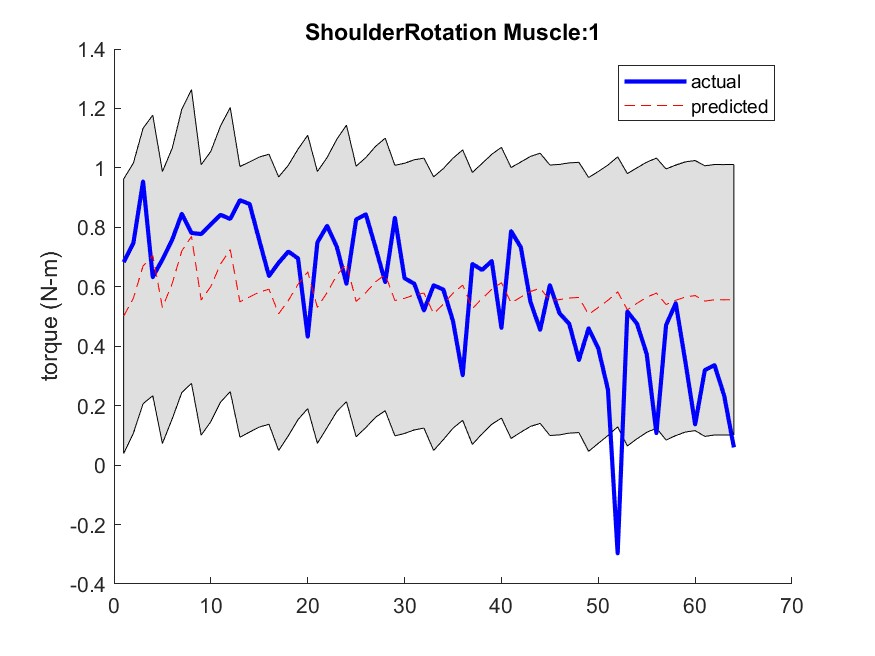
\includegraphics[height=0.15\textheight]{Pictures/Results/GPR/ShoulderRotation_1Parametric.jpg}
        \caption{Shoulder Rotation Parametric}
    \end{subfigure}
    \hfill
    \begin{subfigure}[b]{0.45\linewidth}
        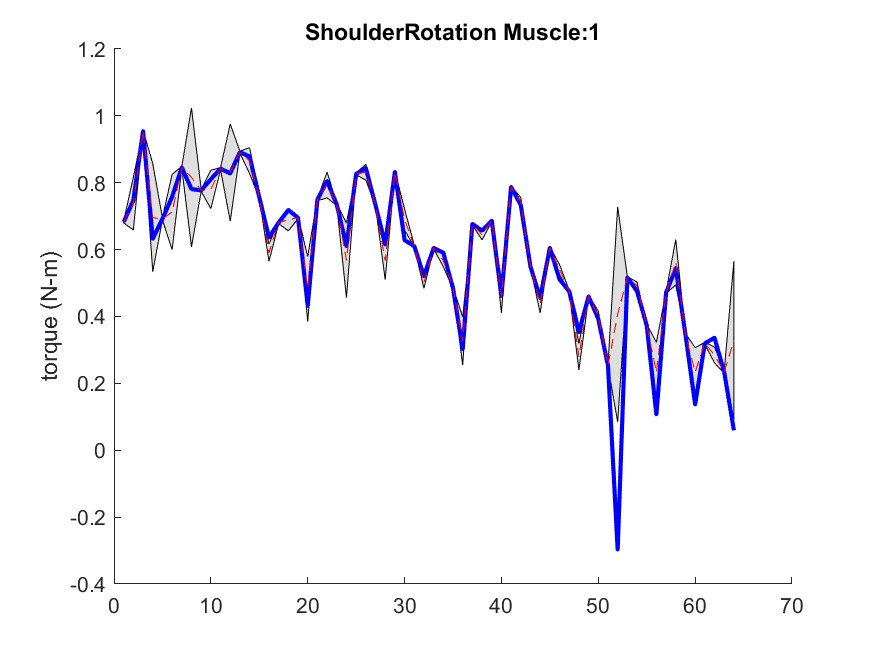
\includegraphics[height=0.15\textheight]{Pictures/Results/GPR/ShoulderRotation_1Semiparametric.jpg}
        \caption{Shoulder Rotation Semi-parametric}
    \end{subfigure}
    
    % Group 4: shoulder elevation
    \begin{subfigure}[b]{0.45\linewidth}
        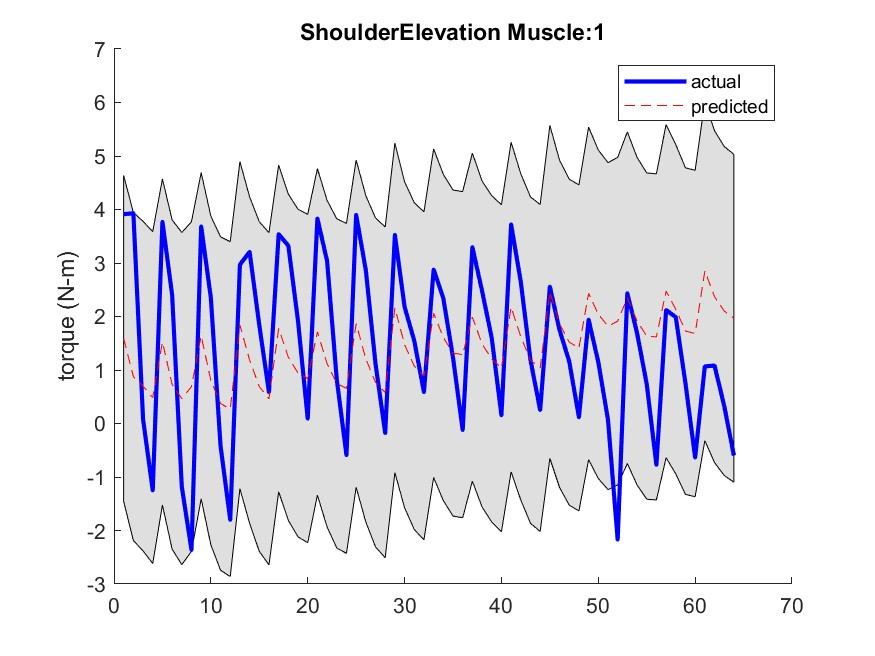
\includegraphics[height=0.15\textheight]{Pictures/Results/GPR/ShoulderElevation_1Parametric.jpg}
        \caption{Shoulder Elevation Parametric}
    \end{subfigure}
    \hfill
    \begin{subfigure}[b]{0.45\linewidth}
        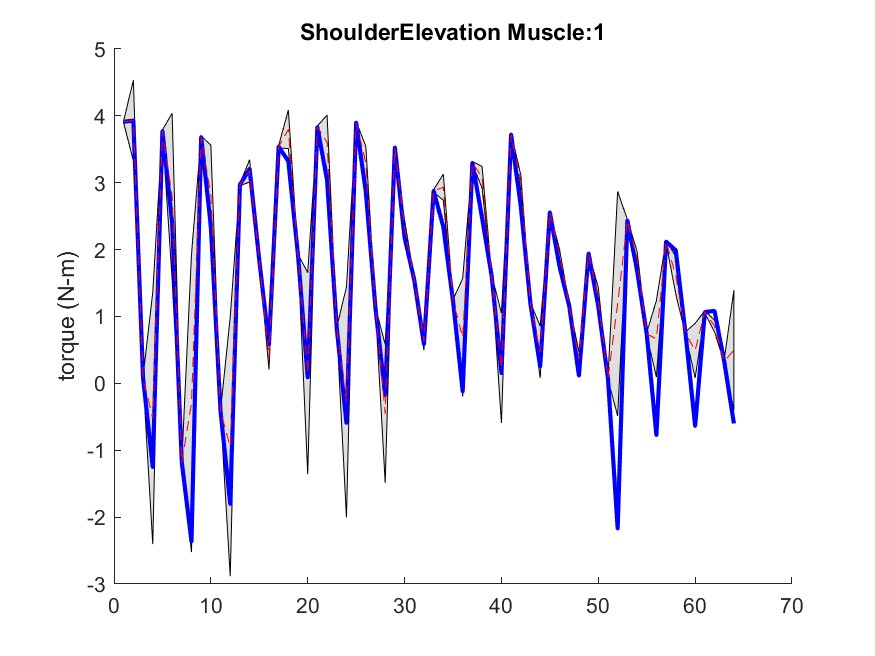
\includegraphics[height=0.15\textheight]{Pictures/Results/GPR/ShoulderElevation_1Semiparametric.jpg}
        \caption{Shoulder Elevation Semi-parametric}
    \end{subfigure}
    
    % Group 5: shoulder elevation plane
    \begin{subfigure}[b]{0.45\linewidth}
        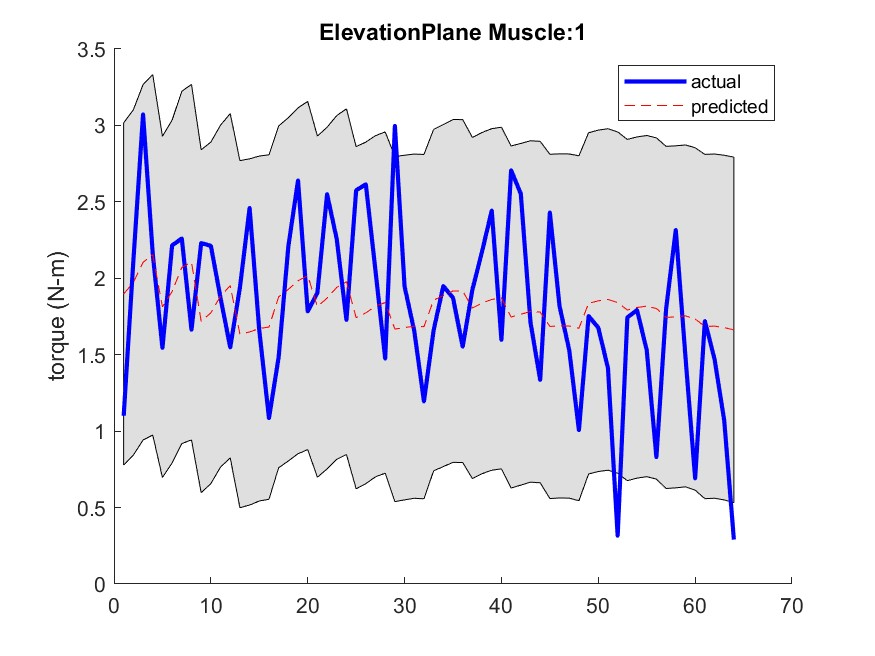
\includegraphics[height=0.15\textheight]{Pictures/Results/GPR/ElevationPlane_1Parametric.jpg}
        \caption{Elevation Plane Parametric}
    \end{subfigure}
    \hfill
    \begin{subfigure}[b]{0.45\linewidth}
        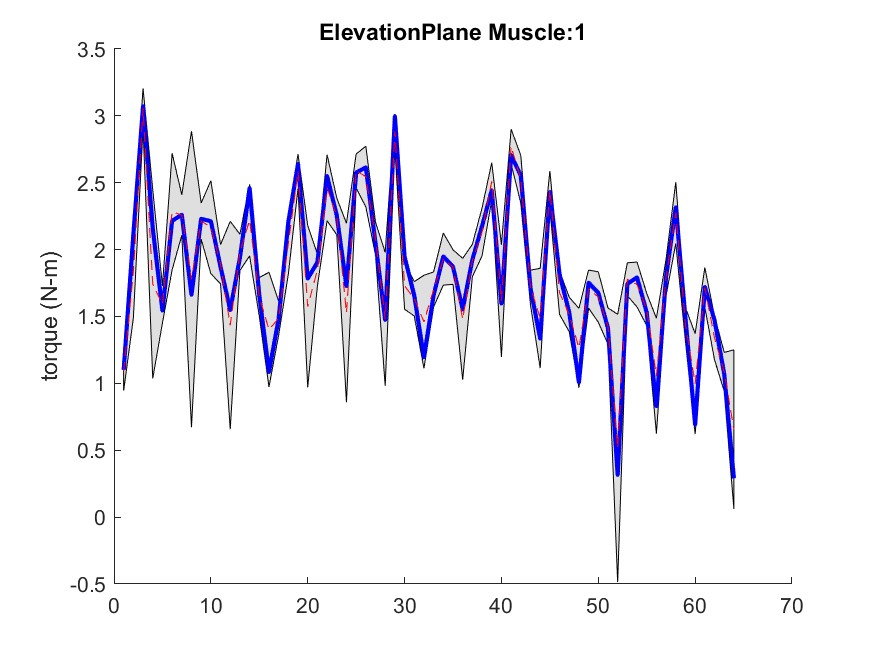
\includegraphics[height=0.15\textheight]{Pictures/Results/GPR/ElevationPlane_1Semiparametric.jpg}
        \caption{Elevation Plane Semi-parametric}
    \end{subfigure}
    
    \caption{Gaussian Process Regression Parametric and Semi-Parametric for Muscle Triceps}
    \label{fig:GPRMuscleTriceps}

\end{figure}